\section{Flow and Diffusion Models}
\label{sec:odes_sdes}
In the previous section, we formalized generative modeling as sampling from a data distribution $\pdata$. Further, we saw that sampling could be achieved via the transformation of samples from a simple distribution $\pinit$, such as the Gaussian $\mathcal{N}(0,I_d)$, to samples from the target distribution $\pdata$. In this section, we describe how the desired transformation can be obtained as the simulation of a suitably constructed differential equation. For example, flow matching and diffusion models involve simulating \themebf{ordinary differential equations} (ODEs) and \themebf{stochastic differential equations} (SDEs), respectively. The goal of this section is therefore to define and construct these generative models as they will be used throughout the remainder of the notes. Specifically, we first define ODEs and SDEs, and discuss their simulation. Second, we describe how to parameterize an ODE/SDE using a deep neural network. This leads to the definition of a flow and diffusion model and the fundamental algorithms to sample from such models. In later sections, we then explore how to train these models.

在前一节中,我们将生成建模形式化为从数据分布$\pdata$中采样。此外,我们看到可以通过将简单分布$\pinit$(如高斯分布$\mathcal{N}(0,I_d)$)的样本转换为目标分布$\pdata$的样本来实现采样。在本节中,我们描述如何通过模拟适当构造的微分方程来获得所需的变换。例如,流匹配和扩散模型分别涉及模拟\themebf{常微分方程}(ODEs)和\themebf{随机微分方程}(SDEs)。因此,本节的目标是定义和构造这些生成模型,因为它们将在笔记的其余部分中使用。具体来说,我们首先定义ODEs和SDEs,并讨论它们的模拟。其次,我们描述如何使用深度神经网络参数化ODE/SDE。这导致了流模型和扩散模型的定义以及从此类模型采样的基本算法。在后面的章节中,我们将探讨如何训练这些模型。

% \paragraph{Note.} We remark that there are other ways to transform $\pinit$ into $\pdata$ other than ODEs/SDEs. We focus on ODEs/SDEs because they represent the current state-of-the-art but just keep in mind that many other ways have been proposed over the course of the history of machine learning offering unique advantages and disadvantages.

\subsection{Flow Models}

We start by defining \themebf{ordinary differential equations (ODEs)}. A solution to an ODE is defined by a \themebf{trajectory}, i.e. a function of the form
\begin{align*}
X: [0,1] \to \R^d, \quad t \mapsto X_t,
\end{align*}
that maps from time $t$ to some location in space $\mathbb{R}^d$. Every ODE is defined by a \themebf{vector field} $u$, i.e. a function of the form
\begin{align*}
u:\mathbb{R}^d\times [0,1]\to \R^d,\quad (x,t)\mapsto u_t(x),
\end{align*}
i.e. for every time $t$ and location $x$ we get a vector $u_t(x)\in\R^d$ specifying a velocity in space (see  \cref{fig:flow}). An ODE imposes a condition on a trajectory: we want a trajectory $X$ that ``follows along the lines'' of the vector field $u_t$, starting at the point $x_0$. We may formalize such a trajectory as being the solution to the equation:

我们首先定义\themebf{常微分方程(ODEs)}。ODE的解由\themebf{轨迹}定义,即形式为
\begin{align*}
X: [0,1] \to \R^d, \quad t \mapsto X_t,
\end{align*}
的函数,它从时间$t$映射到空间$\mathbb{R}^d$中的某个位置。每个ODE都由\themebf{向量场}$u$定义,即形式为
\begin{align*}
u:\mathbb{R}^d\times [0,1]\to \R^d,\quad (x,t)\mapsto u_t(x),
\end{align*}
的函数,即对于每个时间$t$和位置$x$,我们得到一个向量$u_t(x)\in\R^d$,指定空间中的速度(见\cref{fig:flow})。ODE对轨迹施加了一个条件:我们希望轨迹$X$从点$x_0$开始"沿着"向量场$u_t$的线移动。我们可以将这样的轨迹形式化为方程的解:
\begin{subequations}
    \begin{align} 
      \frac{\dd}{\dd t}X_{t} &= u_t(X_t) &&\blacktriangleright\,\,\text{ODE}\label{e:ode_ode}\\
      X_0&= x_0            &&\blacktriangleright\,\,\text{initial conditions}\label{e:ODE_boundary} 
    \end{align}
\end{subequations}
\Cref{e:ode_ode} requires that the derivative of $X_t$ is specified by the direction given by $u_t$. \Cref{e:ODE_boundary} requires that we start at $x_0$ at time $t=0$. We may now ask: if we start at $X_0 = x_0$ at $t=0$, where are we at time $t$ (what is $X_t$)? This question is answered by a function called the \themebf{flow}, which is a solution to the ODE

\Cref{e:ode_ode}要求$X_t$的导数由$u_t$给出的方向指定。\Cref{e:ODE_boundary}要求我们在时间$t=0$时从$x_0$开始。我们现在可以问:如果我们在$t=0$时从$X_0 = x_0$开始,那么在时间$t$时我们在哪里($X_t$是什么)?这个问题由一个称为\themebf{流}的函数回答,它是ODE的解

\begin{subequations}\label{e:flow}
    \begin{align}
    \psi:\R^d\times [0,1]\mapsto& \R^d,\quad (x_0,t)\mapsto \psi_t(x_0)\\
      \frac{\dd}{\dd t}\psi_{t}(x_0) &= u_t(\psi_{t}(x_0)) &&\blacktriangleright\,\, \text{flow ODE}\label{e:flow_flow}\\
      \psi_{0}(x_0)             &= x_0                &&\blacktriangleright\,\,\text{flow initial conditions}\label{e:flow_boundary} 
    \end{align}
\end{subequations}
For a given initial condition $X_0=x_0$, a trajectory of the ODE is recovered via $X_t = \psi_t(X_0)$. Therefore, vector fields, ODEs, and flows are, intuitively, three descriptions of the same object: \textbf{vector fields define ODEs whose solutions are flows}. As with every equation, we should ask ourselves about an ODE: Does a solution exist and if so, is it unique? A fundamental result in mathematics is "yes!" to both, as long we impose weak assumptions on $u_t$:

对于给定的初始条件$X_0=x_0$,ODE的轨迹通过$X_t = \psi_t(X_0)$恢复。因此,向量场、ODEs和流直观上是同一对象的三种描述:\textbf{向量场定义ODEs,其解为流}。就像对每个方程一样,我们应该问自己关于ODE的问题:解是否存在?如果存在,是否唯一?数学中的一个基本结果对这两个问题的答案都是"是的!",只要我们对$u_t$施加弱假设:

\begin{theorem}[Flow existence and uniqueness]
\label{thm:ode_existence_and_uniqueness}
If $u:\R^d\times[0,1]\to\R^d$ is continuously differentiable with a bounded derivative, then the ODE in \eqref{e:flow} has a unique solution given by a flow $\psi_t$. In this case, $\psi_t$ is a \themebf{diffeomorphism} for all $t$, i.e. $\psi_t$ is continuously differentiable with a continuously differentiable inverse $\psi_t^{-1}$.

如果$u:\R^d\times[0,1]\to\R^d$是连续可微的且具有有界导数,那么\eqref{e:flow}中的ODE有由流$\psi_t$给出的唯一解。在这种情况下,$\psi_t$对于所有$t$都是\themebf{微分同胚},即$\psi_t$是连续可微的,且具有连续可微的逆$\psi_t^{-1}$。
\end{theorem}
Note that the assumptions required for the existence and uniqueness of a flow are almost always fulfilled in machine learning, as we use neural networks to parameterize $u_t(x)$ and they always have bounded derivatives. Therefore, \cref{thm:ode_existence_and_uniqueness} should not be a concern for you but rather good news: \textbf{flows exist and are unique solutions to ODEs in our cases of interest.} A proof can be found in \citep{perko2013differential,coddington1956theory}.

注意,在机器学习中,流的存在性和唯一性所需的假设几乎总是满足的,因为我们使用神经网络来参数化$u_t(x)$,而它们总是具有有界导数。因此,\cref{thm:ode_existence_and_uniqueness}不应该是您担心的问题,而应该是好消息:\textbf{在我们感兴趣的情况下,流存在且是ODEs的唯一解。}证明可以在\citep{perko2013differential,coddington1956theory}中找到。

\begin{figure}
    \centering
    \begin{tabular}{ccc}
         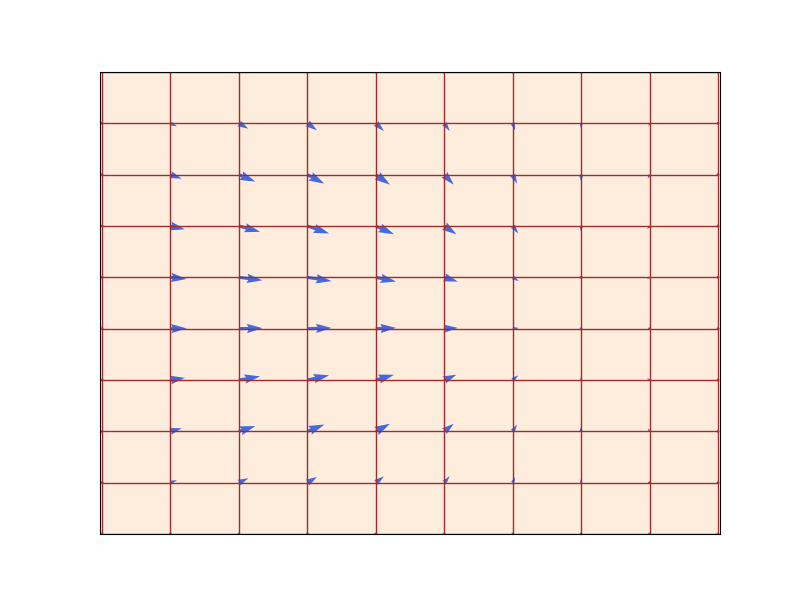
\includegraphics[width=0.3\textwidth]{fm_guide_assets/flow_1.png} &
         % \includegraphics[width=0.22\textwidth]{assets/flow_velocity/flow_v_5.png} &
         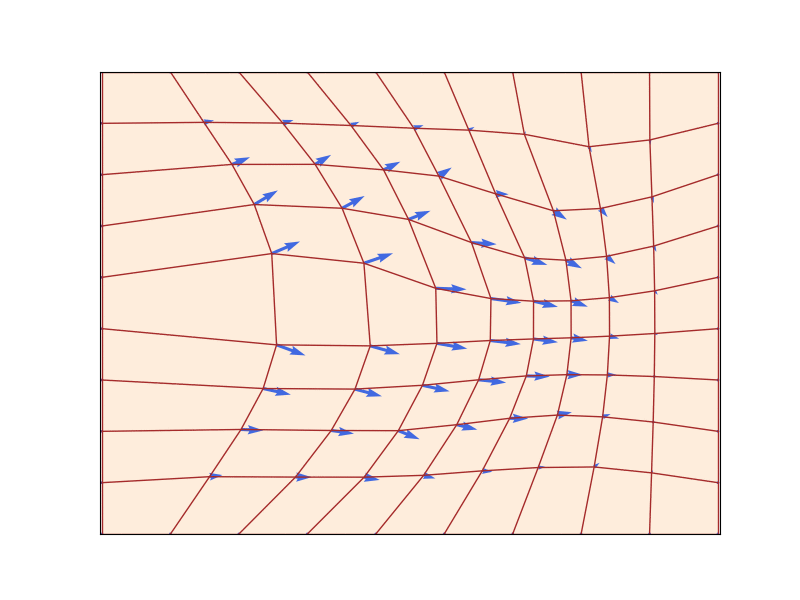
\includegraphics[width=0.3\textwidth]{fm_guide_assets/flow_10.png} &
         % \includegraphics[width=0.22\textwidth]{assets/flow_velocity/flow_v_14.png} &
         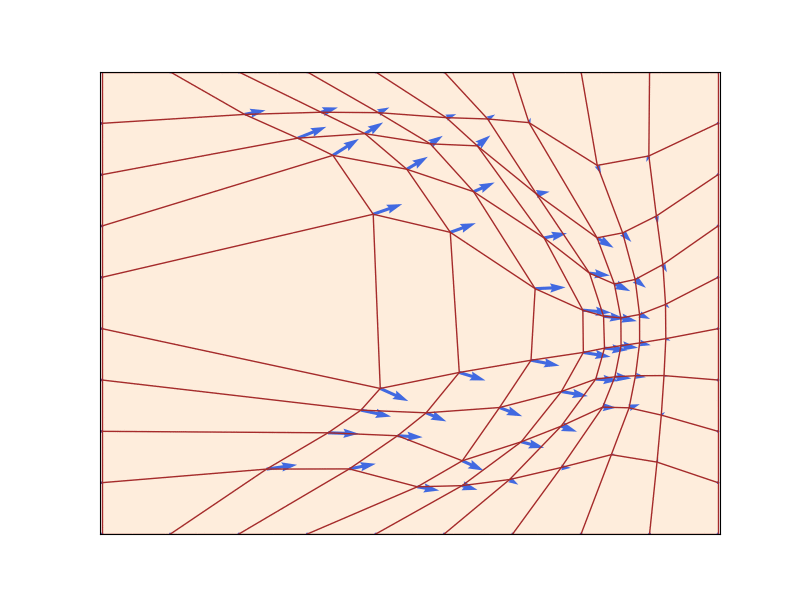
\includegraphics[width=0.3\textwidth]{fm_guide_assets/flow_16.png} 
    \end{tabular}
    \caption{A flow $\psi_t:\Real^d\too \Real^d$ (red square grid) is defined by a velocity field $u_t :\Real^d\too\Real^d$ (visualized with blue arrows) that prescribes its instantaneous movements at all locations (here, $d=2$). We show three different times $t$. As one can see, a flow is a diffeomorphism that "warps" space. Figure from \citep{lipman2024flow}.}
    \label{fig:flow}
    {流$\psi_t:\Real^d\too \Real^d$(红色方格网格)由速度场$u_t :\Real^d\too\Real^d$(用蓝色箭头可视化)定义,该速度场规定了在所有位置的瞬时运动(这里$d=2$)。我们展示了三个不同的时间$t$。如可以看到的,流是一个"扭曲"空间的微分同胚。图来自\citep{lipman2024flow}。}
\end{figure}

\begin{examplebox}[Linear Vector Fields]
Let us consider a simple example of a vector field $u_t(x)$ that is a simple linear function in $x$, i.e. $u_t(x)=-\theta x$ for $\theta>0$. Then the function
\begin{align}
    \label{e:flow_linear_vf}
    \psi_t(x_0) =  \exp\left(-\theta t\right)x_0
\end{align}
defines a flow $\psi$ solving the ODE in \cref{e:flow}. You can check this yourself by checking that $\psi_0(x_0)=x_0$ and computing
\begin{align*}
    \frac{\dd}{\dd t}\psi_t(x_0) \overset{\eqref{e:flow_linear_vf}}{=}\frac{\dd}{\dd t}\left(\exp\left(-\theta t\right)x_0\right)
    \overset{(i)}{=}-\theta\exp\left(-\theta t\right)x_0\overset{\eqref{e:flow_linear_vf}}{=}-\theta\psi_t(x_0)=u_t(\psi_t(x_0)),
\end{align*}
where in (i) we used the chain rule. In \cref{fig:bm_ou_process}, we visualize a flow of this form converging to $0$ exponentially.

让我们考虑一个简单的向量场$u_t(x)$的例子,它是$x$的简单线性函数,即$u_t(x)=-\theta x$,其中$\theta>0$。那么函数
\begin{align}
    \psi_t(x_0) =  \exp\left(-\theta t\right)x_0
\end{align}
定义了一个解决\cref{e:flow}中ODE的流$\psi$。您可以通过检查$\psi_0(x_0)=x_0$并计算
\begin{align*}
    \frac{\dd}{\dd t}\psi_t(x_0) \overset{\eqref{e:flow_linear_vf}}{=}\frac{\dd}{\dd t}\left(\exp\left(-\theta t\right)x_0\right)
    \overset{(i)}{=}-\theta\exp\left(-\theta t\right)x_0\overset{\eqref{e:flow_linear_vf}}{=}-\theta\psi_t(x_0)=u_t(\psi_t(x_0)),
\end{align*}
来自己验证这一点,其中在(i)中我们使用了链式法则。在\cref{fig:bm_ou_process}中,我们可视化了这种形式的流指数收敛到$0$。
\end{examplebox}

\paragraph{Simulating an ODE.}
In general, it is not possible to compute the flow $\psi_t$ explicitly if $u_t$ is not as simple as a linear function. In these cases, one uses \themebf{numerical methods} to simulate ODEs. Fortunately, this is a classical and well researched topic in numerical analysis, and a myriad of powerful methods exist \citep{iserles2009first}. One of the simplest and most intuitive methods is the \themebf{Euler method}. In the Euler method, we initialize with $X_0=x_0$ and update via
\begin{equation}
\label{e:euler_method}
X_{t+h} = X_t + h u_t(X_t)\quad (t=0,h,2h,3h,\dots,1-h)
\end{equation}
where $h=n^{-1}>0$ is a step size hyperparameter with $n \in \Nat$. For this class, the Euler method will be good enough. To give you a taste of a more complex method, let us consider \themebf{Heun's method} defined via the update rule
\begin{alignat*}{3}
    X_{t+h}'&=X_t+hu_t(X_t)\quad &&\blacktriangleright\,\, \text{initial guess of new state}\\
    X_{t+h} &= X_{t} + \frac{h}{2}(u_t(X_t)+u_{t+h}(X_{t+h}'))\quad &&\blacktriangleright\,\,\text{update with average $u$ at current and guessed state}
\end{alignat*}
Intuitively, the Heun's method is as follows: it takes a first guess $X_{t+h}'$ of what the next step could be but corrects the direction initially taken via an updated guess.

\paragraph{模拟ODE。}
一般来说,如果$u_t$不像线性函数那样简单,就不可能明确地计算流$\psi_t$。在这些情况下,我们使用\themebf{数值方法}来模拟ODEs。幸运的是,这是数值分析中一个经典且研究充分的主题,存在无数强大的方法\citep{iserles2009first}。最简单和最直观的方法之一是\themebf{欧拉方法}。在欧拉方法中,我们用$X_0=x_0$初始化,并通过以下方式更新
\begin{equation}
X_{t+h} = X_t + h u_t(X_t)\quad (t=0,h,2h,3h,\dots,1-h)
\end{equation}
其中$h=n^{-1}>0$是步长超参数,$n \in \Nat$。对于这门课程,欧拉方法就足够了。为了让您体验更复杂的方法,让我们考虑通过更新规则定义的\themebf{Heun方法}
\begin{alignat*}{3}
    X_{t+h}'&=X_t+hu_t(X_t)\quad &&\blacktriangleright\,\, \text{新状态的初始猜测}\\
    X_{t+h} &= X_{t} + \frac{h}{2}(u_t(X_t)+u_{t+h}(X_{t+h}'))\quad &&\blacktriangleright\,\,\text{用当前状态和猜测状态的平均$u$更新}
\end{alignat*}
直观地说,Heun方法如下:它首先猜测下一步可能的$X_{t+h}'$,但通过更新的猜测来修正最初采取的方向。

\paragraph{Flow models.} We can now construct a generative model via an ODE. Remember that our goal was to convert a simple distribution $\pinit$ into a complex distribution $\pdata$. The simulation of an ODE is thus a natural choice for this transformation. A \themebf{flow model} is described by the ODE
\begin{align*}
    X_0 &\sim \pinit  &&\blacktriangleright\,\,\text{random initialization} \\
    \frac{\dd}{\dd t}X_t &= u_t^\theta(X_t) &&\blacktriangleright\,\,\text{ODE}
\end{align*}
where the vector field $u_t^\theta$ is a neural network $u_t^\theta$ with parameters $\theta$. For now, we will speak of $u_t^\theta$ as being a generic neural network; i.e. a continuous function $u_t^\theta:\mathbb{R}^d\times [0,1]\to\mathbb{R}^d$ with parameters $\theta$. Later, we will discuss particular choices of neural network architectures. Our goal is to make the endpoint  $X_1$ of the trajectory have distribution $\pdata$, i.e.
\begin{align*}
    X_1 \sim \pdata \quad \Leftrightarrow \quad \psi_1^\theta(X_0)\sim \pdata
\end{align*}
where $\psi_t^\theta$ describes the flow induced by $u_t^\theta$. Note however: although it is called \themeit{flow model}, \textbf{the neural network parameterizes the vector field, not the flow}. In order to compute the flow, we need to simulate the ODE. In \cref{alg:sampling_flow_model}, we summarize the procedure how to sample from a flow model.

\paragraph{流模型。} 我们现在可以通过ODE构造一个生成模型。记住我们的目标是将简单分布$\pinit$转换为复杂分布$\pdata$。因此,ODE的模拟是这种转换的自然选择。\themebf{流模型}由ODE描述
\begin{align*}
    X_0 &\sim \pinit  &&\blacktriangleright\,\,\text{随机初始化} \\
    \frac{\dd}{\dd t}X_t &= u_t^\theta(X_t) &&\blacktriangleright\,\,\text{ODE}
\end{align*}
其中向量场$u_t^\theta$是一个带有参数$\theta$的神经网络$u_t^\theta$。现在,我们将$u_t^\theta$视为一个通用神经网络;即带有参数$\theta$的连续函数$u_t^\theta:\mathbb{R}^d\times [0,1]\to\mathbb{R}^d$。稍后,我们将讨论神经网络架构的特定选择。我们的目标是使轨迹的终点$X_1$具有分布$\pdata$,即
\begin{align*}
    X_1 \sim \pdata \quad \Leftrightarrow \quad \psi_1^\theta(X_0)\sim \pdata
\end{align*}
其中$\psi_t^\theta$描述由$u_t^\theta$诱导的流。但是请注意:尽管它被称为\themeit{流模型},\textbf{神经网络参数化的是向量场,而不是流}。为了计算流,我们需要模拟ODE。在\cref{alg:sampling_flow_model}中,我们总结了如何从流模型采样的过程。

\begin{algorithm}[h]
\caption{Sampling from a Flow Model with Euler method / 使用欧拉方法从流模型中采样}
\label{alg:sampling_flow_model}
\begin{algorithmic}[1]
\REQUIRE Neural network vector field $u_t^\theta$, number of steps $n$ / 神经网络向量场 $u_t^\theta$,步数 $n$
\STATE Set $t=0$ / 设置 $t=0$
\STATE Set step size $h=\frac{1}{n}$ / 设置步长 $h=\frac{1}{n}$
\STATE Draw a sample $X_0\sim \pinit$ / 从 $\pinit$ 中抽取样本 $X_0$
\FOR{$i=1,\dots,n-1$ / 对于 $i=1,\dots,n-1$}
    \STATE $X_{t+h} = X_{t} + h u_t^\theta(X_t)$ / $X_{t+h} = X_{t} + h u_t^\theta(X_t)$
    \STATE Update $t\leftarrow t+h$ / 更新 $t\leftarrow t+h$
\ENDFOR
\RETURN $X_1$ / 返回 $X_1$
\end{algorithmic}
\end{algorithm}

% \paragraph{Flow generative model.}\ph{Potentially leave out this section. We explain the SDE generative model} We can now construct a generative model via flows. A first attempt might be to construct a neural network that approximates a flow $\psi_t$ directly. However, this turns out to be pretty hard as $\psi_t$ has to be a diffeomorphism, which is a hard constraint to enforce on neural networks (if you are interested, you should look up \emph{normalizing flows} \citep{kobyzev2020normalizing}). Instead, it is much simpler to define a neural network that parameterizes a vector field
% \begin{align*}
%     \textbf{Neural Network: }u^\theta:\R^d\times [0,1]\to \R^d, (t,x)\mapsto u_t^\theta(x)\text{  with parameters }\theta
% \end{align*}
% We can equivalently write $\psi_t^\theta$ for the corresponding flow. However, you should always keep in mind that we can only compute $\psi_t^\theta$ by simulating an ODE with the neural network $u_t^\theta$. Therefore, to obtain samples from our \themebf{flow generative model}, the procedure is as follows:
% \begin{align*}
% \textbf{Initialization:}\quad X_0\sim&\pinit \quad  &&(\text{"Initialize with simple distribution, e.g. a Gaussian"})\\
%     \textbf{Simulation:}\quad \frac{\dd}{\dd t}X_t=&u_t^\theta(X_t)\quad &&(\text{"Simulate ODE from 0 to 1, e.g. using Euler method"})\\
%     \textbf{Goal:}\quad X_1 \sim & \pdata \quad &&(\text{"Goal is to make }X_1\text{ have distribution }\pdata\text{"})
% \end{align*}
% Note that the only source of randomness in a flow model is the initial point $X_0\sim \pinit$ - the remaining evolution is deterministic. Further, note that the simulating of the ODE will always incur an error (i.e. we will never be able to compute $\psi_1^\theta$ precisely). However, this is an error that we can usually control by choosing a good ODE solver and simply reducing the step size $h$ in \cref{e:euler_method}.



\subsection{Diffusion Models}
Stochastic differential equations (SDEs) extend the deterministic trajectories from ODEs with \themebf{stochastic} trajectories. A stochastic trajectory is commonly called a \themebf{stochastic process} $(X_t)_{0\leq t\leq 1}$ and is given by
\begin{align*}
    X_t \text{ is a random variable for every } 0\leq t\leq 1\\
    X: [0,1] \to \R^d, \quad t \mapsto X_t\text{ is a random trajectory for every draw of }X
\end{align*}
In particular, when we simulate the same stochastic process twice, we might get different outcomes because the dynamics are designed to be random.

随机微分方程(SDEs)通过\themebf{随机}轨迹扩展了ODEs的确定性轨迹。随机轨迹通常称为\themebf{随机过程}$(X_t)_{0\leq t\leq 1}$,定义为
\begin{align*}
    X_t \text{ 对于每个 } 0\leq t\leq 1\text{ 都是一个随机变量}\\
    X: [0,1] \to \R^d, \quad t \mapsto X_t\text{ 对于}X\text{的每次抽取都是一个随机轨迹}
\end{align*}
特别地,当我们两次模拟同一个随机过程时,我们可能会得到不同的结果,因为动力学被设计为随机的。

\paragraph{Brownian Motion.} SDEs are constructed via a \themebf{Brownian motion} - a fundamental stochastic process that came out of the study physical diffusion processes. You can think of a Brownian motion as a continuous random walk.
\begin{wrapfigure}{r}{0.4\textwidth}
  %\begin{center}
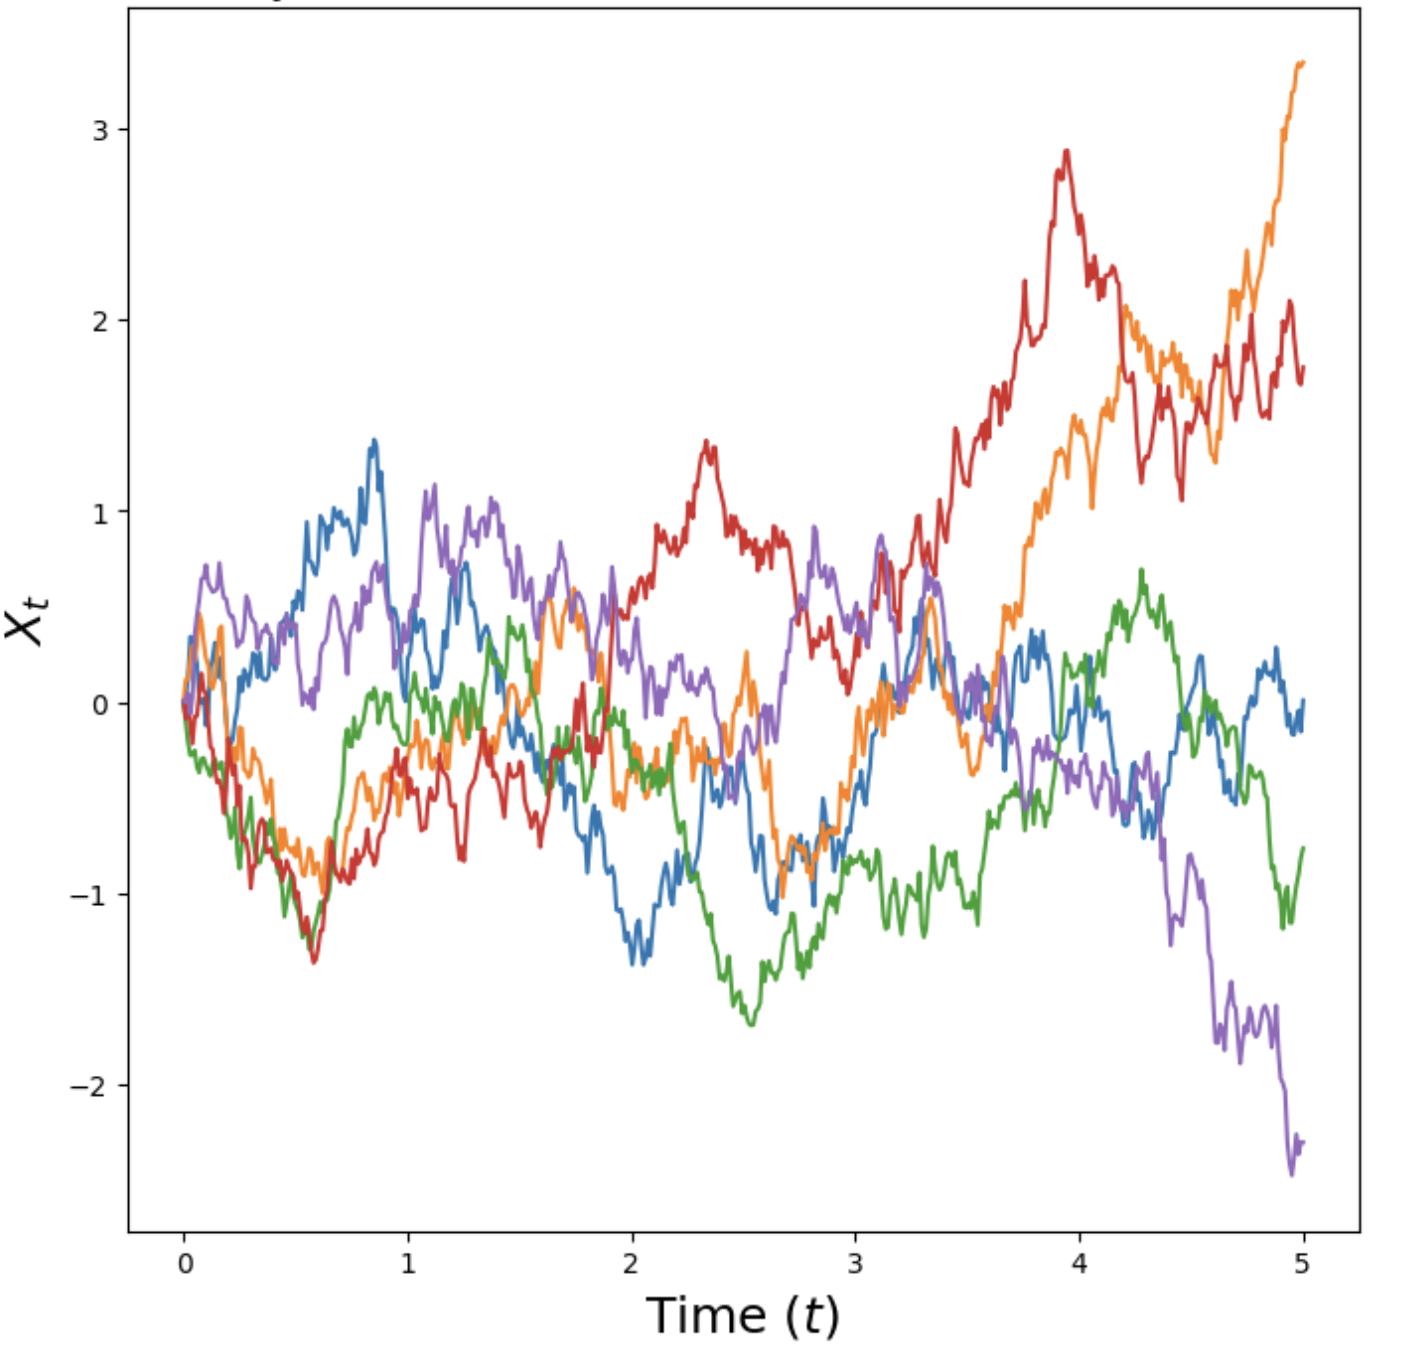
\includegraphics[width=0.4\textwidth]{figures/brownian_motion_sample_paths.png}
  %\end{center}
  \vspace{-20pt}
  \caption{Sample trajectories of a Brownian motion $W_t$ in dimension $d=1$ simulated using \cref{eq:brownian_motion_simulation}.}
  \label{fig:brownian_motion_trajectories}
  \vspace{-10pt}
\end{wrapfigure}
Let us define it: A \themebf{Brownian motion} $W = (W_t)_{0\leq t\leq 1}$ is a stochastic process such that $W_0=0$, the trajectories $t\mapsto W_t$ are continuous, and the following two conditions hold:
\begin{enumerate}
    \item \textbf{Normal increments: }$W_{t}-W_{s}\sim \mathcal{N}(0,(t-s)I_d)$ for all $0\leq s<t$, i.e. increments have a Gaussian distribution with variance increasing linearly in time ($I_d$ is the identity matrix).
    \item \textbf{Independent increments: }For any $0\leq t_0<t_1<\dots <t_n=1$, the increments $W_{t_1}-W_{t_0},\dots,W_{t_n}-W_{t_{n-1}}$ are independent random variables.
\end{enumerate}

Brownian motion is also called a \themebf{Wiener process}, which is why we denote it with a "$W$".\footnote{Nobert Wiener was a famous mathematician who taught at MIT. You can still see his portraits hanging at the MIT math department.} We can easily simulate a Brownian motion approximately with step size $h>0$ by setting $W_0=0$ and updating
\begin{align}
    \label{eq:brownian_motion_simulation}
    W_{t+h} =& W_{t} + \sqrt{h}\epsilon_t,\quad \epsilon_t\sim\mathcal{N}(0,I_d)\quad (t=0,h,2h,\dots,1-h)
\end{align}
In \cref{fig:brownian_motion_trajectories}, we plot a few example trajectories of a Brownian motion.  Brownian motion is as central to the study of stochastic processes as the Gaussian distribution is to the study of probability distributions. From finance to statistical physics to epidemiology, the study of Brownian motion has far reaching applications beyond  machine learning. In finance, for example, Brownian motion is used to model the price of complex financial instruments. Also just as a mathematical construction, Brownian motion is fascinating: For example, while the paths of a Brownian motion are continuous (so that you could draw it without ever lifting a pen), they are infinitely long (so that you would never stop drawing).

\paragraph{布朗运动。} SDEs通过\themebf{布朗运动}构造——这是一个源于物理扩散过程研究的基础随机过程。您可以将布朗运动视为连续随机游走。

让我们定义它:\themebf{布朗运动}$W = (W_t)_{0\leq t\leq 1}$是一个随机过程,满足$W_0=0$,轨迹$t\mapsto W_t$是连续的,并且满足以下两个条件:
\begin{enumerate}
    \item \textbf{正态增量:}对于所有$0\leq s<t$,有$W_{t}-W_{s}\sim \mathcal{N}(0,(t-s)I_d)$,即增量具有方差随时间线性增加的高斯分布($I_d$是单位矩阵)。
    \item \textbf{独立增量:}对于任意$0\leq t_0<t_1<\dots <t_n=1$,增量$W_{t_1}-W_{t_0},\dots,W_{t_n}-W_{t_{n-1}}$是独立随机变量。
\end{enumerate}

布朗运动也称为\themebf{维纳过程},这就是我们用"$W$"表示它的原因。\footnote{诺伯特·维纳是在MIT任教的著名数学家。您仍然可以在MIT数学系看到他的肖像。}我们可以通过设置$W_0=0$并更新来轻松地以步长$h>0$近似模拟布朗运动
\begin{align}
    W_{t+h} =& W_{t} + \sqrt{h}\epsilon_t,\quad \epsilon_t\sim\mathcal{N}(0,I_d)\quad (t=0,h,2h,\dots,1-h)
\end{align}
在\cref{fig:brownian_motion_trajectories}中,我们绘制了布朗运动的几个示例轨迹。布朗运动在随机过程研究中的核心地位,就像高斯分布在概率分布研究中的地位一样。从金融到统计物理再到流行病学,布朗运动的研究在机器学习之外有着深远的应用。例如,在金融领域,布朗运动用于建模复杂金融工具的价格。作为数学构造,布朗运动也很有趣:例如,虽然布朗运动的路径是连续的(因此您可以在不抬笔的情况下绘制它),但它们是无穷长的(因此您永远不会停止绘制)。
%Furhter (2) Any continuous-time Markov process with zero mean and independent, stationary increments is automatically a Brownian motion.

\begin{figure}
    \centering
    \begin{tabular}{ccc}
         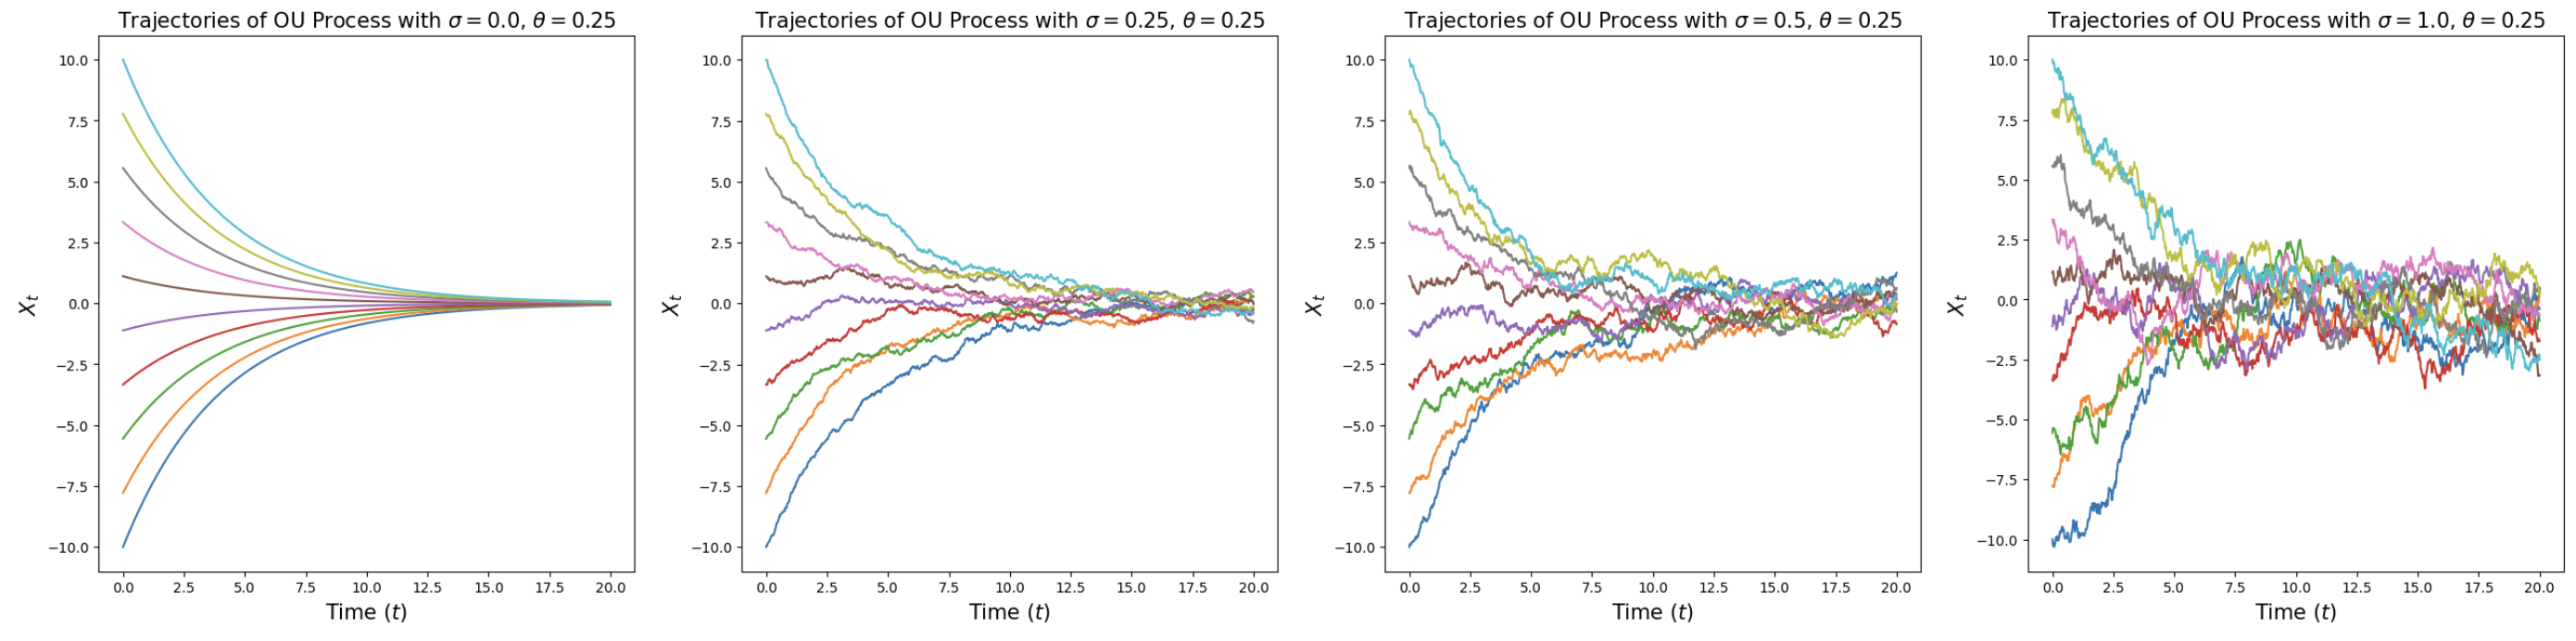
\includegraphics[width=\textwidth]{figures/ou_process.png} &
         % \includegraphics[width=0.22\textwidth]{assets/flow_velocity/flow_v_5.png} &
         % 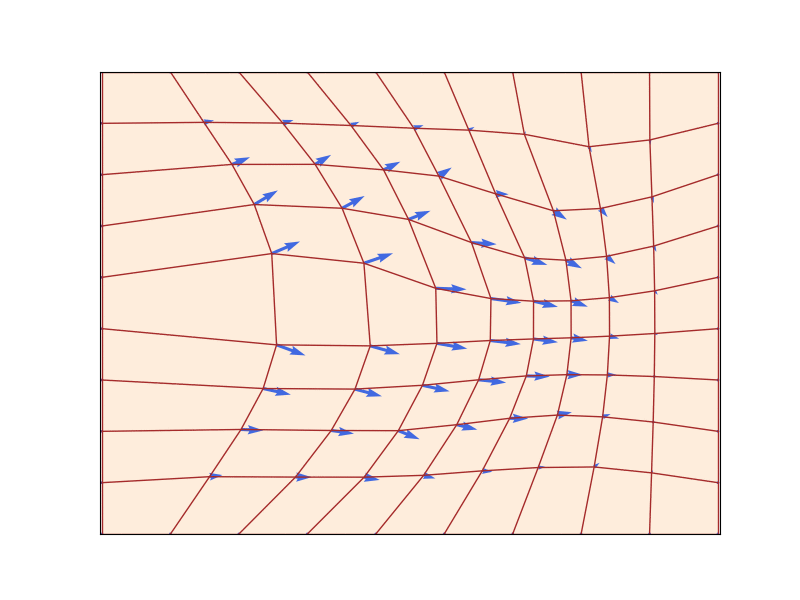
\includegraphics[width=0.3\textwidth]{fm_guide_assets/flow_10.png} &
         % % \includegraphics[width=0.22\textwidth]{assets/flow_velocity/flow_v_14.png} &
         % 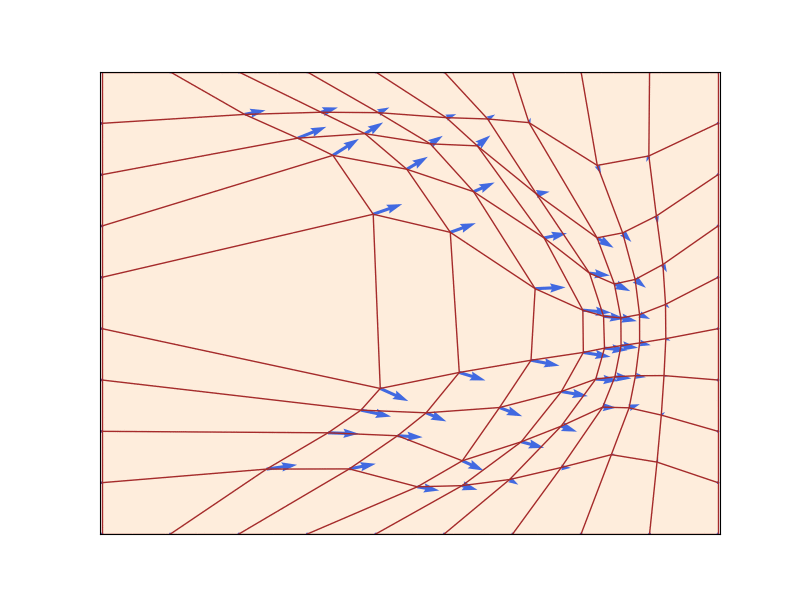
\includegraphics[width=0.3\textwidth]{fm_guide_assets/flow_16.png} 
    \end{tabular}
    \caption{\label{fig:bm_ou_process} Illustration of Ornstein-Uhlenbeck processes (\cref{eq:ohrstein_uhlenbeck_process}) in dimension $d=1$ for $\theta=0.25$ and various choices of $\sigma$ (increasing from left to right). For $\sigma=0$, we recover a flow (smooth, deterministic trajectories) that converges to the origin as $t \to \infty$. For $\sigma>0$ we have random paths which converge towards the Gaussian $\mathcal{N}(0,\frac{\sigma^2}{2\theta})$ as $t\to\infty$. / Ornstein-Uhlenbeck过程(\cref{eq:ohrstein_uhlenbeck_process})在维度$d=1$下的图示,其中$\theta=0.25$和各种$\sigma$选择(从左到右递增)。当$\sigma=0$时,我们恢复了一个流(平滑、确定性轨迹),当$t \to \infty$时收敛到原点。当$\sigma>0$时,我们有随机路径,当$t\to\infty$时收敛到高斯分布$\mathcal{N}(0,\frac{\sigma^2}{2\theta})$。}
\end{figure} 

\paragraph{From ODEs to SDEs.} The idea of an SDE is to extend the deterministic dynamics of an ODE by adding stochastic dynamics driven by a Brownian motion. Because everything is stochastic, we may no longer take the derivative as in \cref{e:ode_ode}. Hence, we need to find an \textbf{equivalent formulation of ODEs that does not use derivatives}. For this, let us therefore rewrite trajectories $(X_t)_{0\leq t\leq 1}$ of an ODE as follows:
\begin{alignat*}{3}
    \frac{\dd}{\dd t} X_t &=  u_t(X_t) \quad &&\blacktriangleright\,\,\text{expression via derivatives}\\
    \overset{(i)}{\Leftrightarrow} \quad  \frac{1}{h}\left(X_{t+h}-X_{t}\right)&=u_t(X_t) + R_t(h)&&\\
\Leftrightarrow \quad X_{t+h} &= X_{t}+hu_t(X_t) + hR_t(h)\quad &&\blacktriangleright\,\,\text{expression via infinitesimal updates}
\end{alignat*}
where  $R_t(h)$ describes a negligible function for small $h$, i.e. such that $\lim\limits_{h\to 0}R_t(h)=0$, and in $(i)$ we simply use the definition of derivatives. The derivation above simply restates what we already know: A trajectory $(X_t)_{0 \le t \le 1}$ of an ODE takes, at every timestep, a small step in the direction $u_t(X_t)$. We may now amend the last equation to make it stochastic: A trajectory $(X_t)_{0 \le t \le 1}$ of an SDE takes, at every timestep, a small step in the direction $u_t(X_t)$ \themeit{plus} some contribution from a Brownian motion:
\begin{align}
    \label{e:infinitesimal_updates_sdes}
    X_{t+h} = X_{t}+\underbrace{hu_t(X_t)}_{\text{deterministic}} + \sigma_t\underbrace{(W_{t+h}-W_{t})}_{\text{stochastic}}+\underbrace{hR_t(h)}_{\text{error term}}
\end{align}
where $\sigma_t\geq 0$ describes the \themebf{diffusion coefficient} and $R_t(h)$ describes a stochastic error term such that the standard deviation $\mathbb{E}[\|R_t(h)\|^2]^{1/2}\to 0$ goes to zero for $h\to 0$. The above describes a \themebf{stochastic differential equation (SDE)}. It is common to denote it in the following symbolic notation:
\begin{subequations}\label{e:sde_generic}
    \begin{align} 
      \dd X_t &= u_t(X_t)\dd t + \sigma_t\dd W_t &&\blacktriangleright\,\,\text{SDE}\\
      X_0 &= x_0               &&\blacktriangleright\,\,\text{initial condition}
    \end{align}
\end{subequations}
However, always keep in mind that the "$\dd X_t$"-notation above is a purely informal notation of \cref{e:infinitesimal_updates_sdes}. Unfortunately, SDEs do not have a flow map $\phi_t$ anymore. This is because the value $X_t$ is not fully determined by $X_0\sim \pinit$ anymore as the evolution itself is stochastic. Still, in the same way as for ODEs, we have:
\paragraph{从ODEs到SDEs。} SDE的思想是通过添加由布朗运动驱动的随机动力学来扩展ODE的确定性动力学。因为一切都是随机的,我们不能再像\cref{e:ode_ode}中那样取导数。因此,我们需要找到\textbf{不使用导数的ODEs等价表述}。为此,让我们将ODE的轨迹$(X_t)_{0\leq t\leq 1}$重写如下:
\begin{alignat*}{3}
    \frac{\dd}{\dd t} X_t &=  u_t(X_t) \quad &&\blacktriangleright\,\,\text{通过导数表达}\\
    \overset{(i)}{\Leftrightarrow} \quad  \frac{1}{h}\left(X_{t+h}-X_{t}\right)&=u_t(X_t) + R_t(h)&&\\
\Leftrightarrow \quad X_{t+h} &= X_{t}+hu_t(X_t) + hR_t(h)\quad &&\blacktriangleright\,\,\text{通过无穷小更新表达}
\end{alignat*}
其中$R_t(h)$描述一个对小$h$可忽略的函数,即满足$\lim\limits_{h\to 0}R_t(h)=0$,在$(i)$中我们只是使用导数的定义。上面的推导只是重述了我们已经知道的内容:ODE的轨迹$(X_t)_{0 \le t \le 1}$在每个时间步都沿方向$u_t(X_t)$迈出一小步。我们现在可以修改最后一个方程使其随机化:SDE的轨迹$(X_t)_{0 \le t \le 1}$在每个时间步都沿方向$u_t(X_t)$迈出一小步\themeit{加上}来自布朗运动的一些贡献:
\begin{align}
    X_{t+h} = X_{t}+\underbrace{hu_t(X_t)}_{\text{确定性}} + \sigma_t\underbrace{(W_{t+h}-W_{t})}_{\text{随机性}}+\underbrace{hR_t(h)}_{\text{误差项}}
\end{align}
其中$\sigma_t\geq 0$描述\themebf{扩散系数},$R_t(h)$描述随机误差项,使得标准差$\mathbb{E}[\|R_t(h)\|^2]^{1/2}\to 0$当$h\to 0$时趋于零。上述描述了\themebf{随机微分方程(SDE)}。通常用以下符号记号表示:
\begin{subequations}
    \begin{align} 
      \dd X_t &= u_t(X_t)\dd t + \sigma_t\dd W_t &&\blacktriangleright\,\,\text{SDE}\\
      X_0 &= x_0               &&\blacktriangleright\,\,\text{初始条件}
    \end{align}
\end{subequations}
但是,请始终记住上面的"$\dd X_t$"记号只是\cref{e:infinitesimal_updates_sdes}的纯粹非正式记号。不幸的是,SDEs不再有流映射$\phi_t$。这是因为$X_t$的值不再完全由$X_0\sim \pinit$确定,因为演化本身是随机的。尽管如此,与ODEs相同的方式,我们有:
\begin{theorem}[SDE Solution Existence and Uniqueness]
    
\label{thm:sde_existence_and_uniqueness}
If $u:\R^d\times[0,1]\to\R^d$ is continuously differentiable with a bounded derivative and $\sigma_t$ is continuous, then the SDE in \eqref{e:sde_generic} has a solution given by the unique stochastic process $(X_t)_{0\leq t\leq 1}$ satisfying \cref{e:infinitesimal_updates_sdes}.
\\如果$u:\R^d\times[0,1]\to\R^d$是连续可微的且有有界导数,$\sigma_t$是连续的,那么\eqref{e:sde_generic}中的SDE有一个解,由满足\cref{e:infinitesimal_updates_sdes}的唯一随机过程$(X_t)_{0\leq t\leq 1}$给出。
\end{theorem}
If this was a stochastic calculus class, we would spend several lectures proving this theorem and constructing SDEs with full mathematical rigor, i.e. constructing a Brownian motion from first principles and constructing the process $X_{t}$ via \themebf{stochastic integration}. As we focus on machine learning in this class, we refer to \citep{mao2007stochastic} for a more technical treatment. Finally, note that every ODE is also an SDE - simply with a vanishing diffusion coefficient $\sigma_t=0$. Therefore, for the remainder of this class, \textbf{when we speak about SDEs, we consider ODEs as a special case}.


如果这是随机微积分课程,我们会花几节课来证明这个定理并以完全的数学严格性构造SDEs,即从第一原理构造布朗运动并通过\themebf{随机积分}构造过程$X_{t}$。由于我们在这门课中专注于机器学习,我们参考\citep{mao2007stochastic}以获得更技术性的处理。最后,注意每个ODE也是SDE——只是扩散系数$\sigma_t=0$消失了。因此,在本课程的其余部分,\textbf{当我们谈论SDEs时,我们将ODEs视为特殊情况}。
% \begin{remarkbox}[A Note on Formality]
% If this was a stochastic calculus class, we would spend more time constructing SDEs with full mathematical rigor, i.e. constructing a Brownian motion from first principles and constructing the process $X_{t}$ via \emph{stochastic integrals}. \ee{Revise: Those of you familiar with stochastic calculus will note that our discussion of SDEs has thus far been quite informal. For example, we have technically not actually shown that a Brownian motion even exists. If this were a class on stochastic calculus, we might proceed more formally, by e.g., constructing a Brownian motion and then arriving at SDEs via the notion of a \themeit{stochastic integral}. Nevertheless, we feel that this extra machinery is overly cumbersome for the need at hand, and have therefore opted to take a more direct approach.}
% \end{remarkbox}

\begin{examplebox}[Ornstein-Uhlenbeck Process]
Let us consider a constant diffusion coefficient $\sigma_t=\sigma\geq 0$ and a constant linear drift $u_t(x)=-\theta x$ for $\theta>0$, yielding the SDE
\begin{align}
\label{eq:ohrstein_uhlenbeck_process}
\dd X_t = -\theta X_t\dd t + \sigma dW_t.
\end{align} 
A solution $(X_t)_{0 \le t \le 1}$ to the above SDE is known as an \themebf{Ornstein-Uhlenbeck (OU) process}. We visualize it in \cref{fig:bm_ou_process}. The vector field $-\theta x$ pushes the process back to its center $0$ (as I always go the inverse direction of where I am), while the diffusion coefficient $\sigma$ always adds more noise. This process converges towards a Gaussian distribution $\mathcal{N}(0,\sigma^2)$ if we simulate it for $t\to \infty$. Note that for $\sigma=0$, we have a flow with linear vector field that we have studied in \cref{e:flow_linear_vf}.

让我们考虑常数扩散系数$\sigma_t=\sigma\geq 0$和常数线性漂移$u_t(x)=-\theta x$(其中$\theta>0$),得到SDE
\begin{align}
\dd X_t = -\theta X_t\dd t + \sigma dW_t.
\end{align} 
上述SDE的解$(X_t)_{0 \le t \le 1}$被称为\themebf{Ornstein-Uhlenbeck(OU)过程}。我们在\cref{fig:bm_ou_process}中可视化了它。向量场$-\theta x$将过程推回到其中心$0$(因为我总是朝着我所在位置的相反方向移动),而扩散系数$\sigma$总是增加更多噪声。如果我们对$t\to \infty$进行模拟,这个过程会收敛到高斯分布$\mathcal{N}(0,\sigma^2)$。注意,对于$\sigma=0$,我们有一个具有线性向量场的流,我们在\cref{e:flow_linear_vf}中研究过。
\end{examplebox}


\paragraph{Simulating an SDE.} If you struggle with the abstract definition of an SDE so far, then don't worry about it. A more intuitive way of thinking about SDEs is given by answering the question: How might we simulate an SDE? The simplest such scheme is known as the \themebf{Euler-Maruyama method}, and is essentially to SDEs what the Euler method is to ODEs. Using the Euler-Maruyama method, we initialize $X_0=x_0$ and update iteratively via
\begin{align}
\label{e:euler_method_sdes}
    X_{t+h} = X_{t}+hu_t(X_t) + \sqrt{h}\sigma_t\epsilon_t,\quad \quad \epsilon_t \sim \mathcal{N}(0,I_d)
\end{align}
where $h=n^{-1}>0$ is a step size hyperparameter for $n \in \Nat$. In other words, to simulate using the Euler-Maruyama method, we take a small step in the direction of $u_t(X_t)$ as well as add a little bit of Gaussian noise scaled by $\sqrt{h}\sigma_t$. When simulating SDEs in this class (such as in the accompanying labs), we will usually stick to the Euler-Maruyama method.

\paragraph{模拟SDE。} 如果您到目前为止对SDE的抽象定义感到困惑,那么不要担心。通过回答这个问题,可以给出思考SDEs的更直观方法:我们如何模拟SDE?最简单的这种方案被称为\themebf{Euler-Maruyama方法},它本质上对SDEs的作用就像欧拉方法对ODEs的作用一样。使用Euler-Maruyama方法,我们用$X_0=x_0$初始化并通过以下方式迭代更新
\begin{align}
    X_{t+h} = X_{t}+hu_t(X_t) + \sqrt{h}\sigma_t\epsilon_t,\quad \quad \epsilon_t \sim \mathcal{N}(0,I_d)
\end{align}
其中$h=n^{-1}>0$是$n \in \Nat$的步长超参数。换句话说,要使用Euler-Maruyama方法进行模拟,我们沿$u_t(X_t)$方向迈出一小步,并添加一点由$\sqrt{h}\sigma_t$缩放的高斯噪声。在本课程中模拟SDEs时(例如在随附的实验中),我们通常会坚持使用Euler-Maruyama方法。

\begin{algorithm}[h]
\caption{Sampling from a Diffusion Model (Euler-Maruyama  method)}
\label{alg:sampling_diffusion_model}
\begin{algorithmic}[1]
\REQUIRE Neural network $u_t^\theta$, number of steps $n$, diffusion coefficient $\sigma_t$
\STATE Set $t=0$
\STATE Set step size $h=\frac{1}{n}$
\STATE Draw a sample $X_0\sim \pinit$
\FOR{$i=1,\dots,n-1$}
    \STATE Draw a sample $\epsilon\sim \mathcal{N}(0,I_d)$
    \STATE $X_{t+h} = X_{t} + h u_t^\theta(X_t)+\sigma_t\sqrt{h}\epsilon$
    \STATE Update $t\leftarrow t+h$
\ENDFOR
\RETURN $X_1$
\end{algorithmic}
\end{algorithm}

\paragraph{Diffusion Models.} We can now construct a generative model via an SDE in the same way as we did for ODEs. Remember that our goal was to convert a simple distribution $\pinit$ into a complex distribution $\pdata$. Like for ODEs, the simulation of an SDE randomly initialized with $X_0\sim \pinit$ is a natural choice for this transformation. To parameterize this SDE, we can simply parameterize its central ingredient - the vector field $u_t$ - a neural network $u_t^\theta$. A \themebf{diffusion model} is thus given by
\begin{align*}
    \dd X_t &= u_t^\theta(X_t)\dd t + \sigma_t \dd W_t &&\blacktriangleright\,\,\text{SDE}\\
    X_0 &\sim \pinit  &&\blacktriangleright\,\,\text{random initialization}
    \end{align*}
In \cref{alg:sampling_diffusion_model}, we describe the procedure by which to sample from a diffusion model with the Euler-Maruyama method. We summarize the results of this section as follows.

\paragraph{扩散模型。} 我们现在可以通过SDE构造生成模型,就像我们对ODEs所做的那样。记住我们的目标是将简单分布$\pinit$转换为复杂分布$\pdata$。像对ODEs一样,用$X_0\sim \pinit$随机初始化的SDE模拟是这种转换的自然选择。为了参数化这个SDE,我们可以简单地参数化其核心成分——向量场$u_t$——一个神经网络$u_t^\theta$。因此,\themebf{扩散模型}由以下给出
\begin{align*}
    \dd X_t &= u_t^\theta(X_t)\dd t + \sigma_t \dd W_t &&\blacktriangleright\,\,\text{SDE}\\
    X_0 &\sim \pinit  &&\blacktriangleright\,\,\text{随机初始化}
    \end{align*}
在\cref{alg:sampling_diffusion_model}中,我们描述了使用Euler-Maruyama方法从扩散模型采样的过程。我们总结本节的结果如下。
\begin{summarybox}[SDE generative model] Throughout this document, a \themebf{diffusion model} consists of a neural network $u_t^\theta$ with parameters $\theta$ that parameterize a vector field and a fixed  diffusion coefficient $\sigma_t$:
\begin{align*}
    \textbf{\sffamily Neural network: }&u^\theta:\R^d\times [0,1]\to \R^d,\,\, (x,t)\mapsto u_t^\theta(x)\text{  with parameters }\theta\\
    \textbf{\sffamily Fixed: }&\sigma_t:[0,1]\to [0,\infty),\,\, t\mapsto \sigma_t
\end{align*}
To obtain samples from our SDE model (i.e. generate objects), the procedure is as follows:
\begin{align*}
\textbf{\sffamily Initialization:}\quad X_0&\sim\pinit \quad  &&\blacktriangleright\,\,\text{Initialize with simple distribution, e.g. a Gaussian}\\
    \textbf{\sffamily Simulation:}\quad \dd X_t &= u_t^\theta(X_t)\dd t + \sigma_t\dd W_t\quad &&\blacktriangleright\,\,\text{Simulate SDE from 0 to 1}\\
    \textbf{\sffamily Goal:}\quad X_1 &\sim  \pdata \quad &&\blacktriangleright\,\,\text{Goal is to make $X_1$ have distribution $\pdata$}
\end{align*}
A diffusion model with $\sigma_t=0$ is a \themebf{flow model}.
\label{summary:diffusion_model}

在整个文档中,\themebf{扩散模型}由一个带有参数$\theta$的神经网络$u_t^\theta$(参数化向量场)和一个固定的扩散系数$\sigma_t$组成:
\begin{align*}
    \textbf{\sffamily 神经网络:}&u^\theta:\R^d\times [0,1]\to \R^d,\,\, (x,t)\mapsto u_t^\theta(x)\text{  带参数}\theta\\
    \textbf{\sffamily 固定的:}&\sigma_t:[0,1]\to [0,\infty),\,\, t\mapsto \sigma_t
\end{align*}
要从我们的SDE模型获得样本(即生成对象),过程如下:
\begin{align*}
\textbf{\sffamily 初始化:}\quad X_0&\sim\pinit \quad  &&\blacktriangleright\,\,\text{用简单分布初始化,例如高斯分布}\\
    \textbf{\sffamily 模拟:}\quad \dd X_t &= u_t^\theta(X_t)\dd t + \sigma_t\dd W_t\quad &&\blacktriangleright\,\,\text{从0到1模拟SDE}\\
    \textbf{\sffamily 目标:}\quad X_1 &\sim  \pdata \quad &&\blacktriangleright\,\,\text{目标是使$X_1$具有分布$\pdata$}
\end{align*}
$\sigma_t=0$的扩散模型是\themebf{流模型}。
\end{summarybox}

